\documentclass{standalone}

\usepackage{tikz}
\usepackage{tkz-euclide}
\usetikzlibrary{calc}
\usetikzlibrary{positioning}
\usetikzlibrary{arrows.meta}
\usetikzlibrary{shapes,snakes}

\usepackage{times}

\definecolor{myblue}{rgb}{0.0,0.5,0.8}

\begin{document}
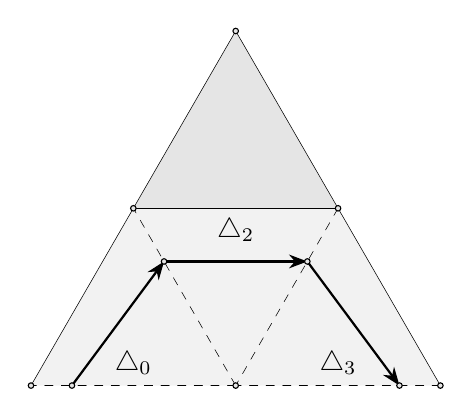
\begin{tikzpicture}[%
  >={Stealth[scale=1.0]},
  face/.style={star, star points = 8},
  scale=1.3,
]

  \tkzDefPoint(0.0, 0.0){v0}
  \tkzDefPoint(2.0, 0.0){v1}
  \tkzDefPoint(1.0, -1.7321){v2}
  \tkzDefPoint(1.0, 1.7321){v3}
  \tkzDefPoint(3.0, -1.7321){v4}
  \tkzDefPoint(-1.0, -1.7321){v5}

  \tkzDefPointOnLine[pos=0.2](v5,v2)\tkzGetPoint{e0}
  \tkzDefPointOnLine[pos=0.3](v0,v2)\tkzGetPoint{e1}
  \tkzDefPointOnLine[pos=0.3](v1,v2)\tkzGetPoint{e2}
  \tkzDefPointOnLine[pos=0.8](v2,v4)\tkzGetPoint{e3}

  \tkzFillPolygon[color=black!5](v0,v1,v2)
  \tkzFillPolygon[color=black!10](v0,v1,v3)
  \tkzFillPolygon[color=black!5](v1,v2,v4)
  \tkzFillPolygon[color=black!5](v2,v0,v5)

  \tkzDrawSegments(v0,v1 v0,v3 v3,v1 v1,v4 v0,v5)
  \tkzDrawSegments[dashed](v1,v2 v2,v0 v4,v2 v2,v5)
  \tkzDrawPoints(v0,v1,v2,v3,v4,v5)

  \tkzDrawSegments[thick,->](e0,e1 e1,e2 e2,e3)
  \tkzDrawPoints(e0,e1,e2,e3)

  \tkzLabelSegments[above](v5,v2){$\triangle_0$}
  \tkzLabelSegments[above](v4,v2){$\triangle_3$}
  \tkzLabelSegments[below](v0,v1){$\triangle_2$}

\end{tikzpicture}
\end{document}
